\documentclass[12pt, letterpaper]{article}

\usepackage{amssymb}
\usepackage{amsmath}
\usepackage{latexsym}
\usepackage[margin=1in]{geometry}
\usepackage{fancyhdr}
\usepackage{listings}

\usepackage{graphicx}
\graphicspath{{../Pictures/}}
\usepackage{float}

\lhead{Darsh Shah \& Luv Iyer}
\chead{ESE 531 Final Project}
\rhead{April 24, 2018}

\title{ESE 531 Final Project}
\author{Darsh Shah, EE '19 
\\ Luv Iyer, EE '20 \\ Dr. Tania Khanna, University of Pennsylvania}
\date{April 24, 2018}

\begin{document}
	\maketitle
	
	\newpage
	
	\section{Part A - Adaptive Notch Filter}
	
	Just stuff in the works....just to give you the idea of what the document can look like, and how we would go about putting pictures in and stuff....
	
	\subsection{A}
	
	We see with our parameters, $a$ converges:
	
	\begin{figure}[H]
		\centering
		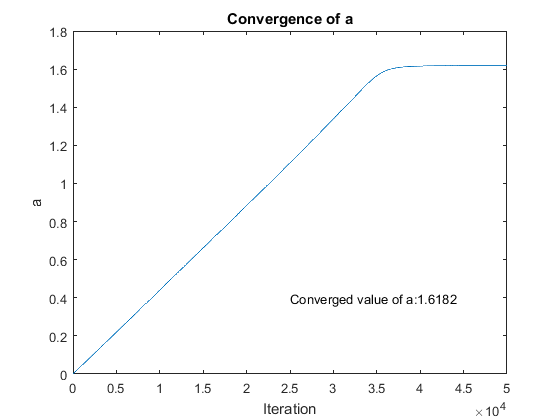
\includegraphics[width=\textwidth]{pAaconvergencea}
		
		\caption{a converges after many iterations}	
	\end{figure}
	
	We did a bunch of stuff and we see that we were able to make a an adaptive notch filter that filters out the desired frequency.
	
	\begin{figure}[H]
		\centering
		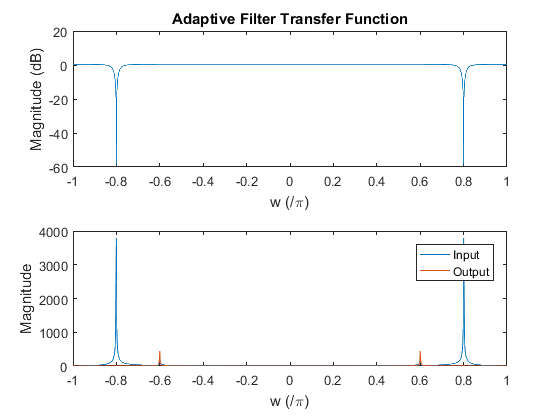
\includegraphics[width=\textwidth]{pAiot}
		
		\caption{Adaptive notch filter filters out noise frequency 0.4.}	
	\end{figure}

	Here is the code for this section...More to come
	
	\begin{lstlisting}
% Adaptive notch
clear; clc;

% Calibrate initial values to specify attributes of adaptive filter 
r = 0.95;
mu = 1E-6; % This mu should be small enough for a to converge
N = 50000; 

% Initialize signal arrays for use in algorithm
e = zeros(1,N);
y = zeros(1,N);
a = zeros(1,N);
w = linspace(-pi, pi, N);
z = exp(1i*w); % Used for transfer function calculation

n = 1:N;
f_desired = 0.3;
f_noise = 0.4;
desired = cos(2*pi*f_desired*n);    % Clean signal 
noise = 10*cos(2*pi*f_noise*n);   % Strong interference 
x = desired + noise;          % Combined input signal

for i = 3:N-1
e(i) = x(i)+a(i)*x(i-1)+x(i-2);
y(i) = e(i)-r*a(i)*y(i-1)-(r^2)*y(i-2);
if ((a(i)>=-2)&&(a(i)<2)) 
a(i+1) = a(i)-mu*y(i)*x(i-1);
else 
a(i+1) = 0;
end 
end


% Compute the transfer function of the filter
H_adaptive = (1+a(end)*z.^(-1)+z.^(-2))./(1+r*a(end)*z.^(-1)+r^2*z.^(-2));

subplot(2,1,1)
plot(w/pi, 20*log10(abs(H_adaptive)))
title('Adaptive Filter Transfer Function');
xlabel('w (/\pi)'); ylabel('Magnitude (dB)');

subplot(2,1,2)
% Take the fft of the final 1000 samples of x and y. This data will
% reflect that the noise frequency has been filtered out.
H_x = fftshift(fft(x(end-1000: end), 1001));
H_y = fftshift(fft(y(end-1000:end), 1001));

% Frequency samples should correspond to length of fft
w_ = linspace(-pi, pi, 1001)/pi;  
plot(w_, abs(H_x));
hold on;
plot(w_, abs(H_y));
xlabel('w (/\pi)'); ylabel('Magnitude');
legend('Input', 'Output');

% Plot the value of a to show convergence
figure(2)
plot(a)
title('Convergence of a');
xlabel('Iteration'); ylabel('a');
text(25000, .4, strcat('Converged value of a: ', num2str(a(end))));
	\end{lstlisting}
	
\end{document}

